This section presents an architecture and execution environment to put together 
semantics and existing techniques for dealing with data streams in real-time. 
It is based on the architecture defined in~\cite{BigDataManing} by Nathan Marz that defines 
a general data system as a system that runs arbitrary functions on arbitrary data. This definition 
follows the next equation $query=f(all\,data)$ which is the basis of all systems. The Lambda 
Architectures defines then a clear set of principles to build robust and scalable data 
systems obeying the aforementioned equation. Basically three main design principles 
can be found:
\begin{itemize}
 \item Human fault-tolerance. The system is unsusceptible to data loss or data corruption because at scale it could be irreparable.
 \item Data immutability. Data is stored in a raw form to be immutable and for perpetuity.
 \item Re-computation. Following the two previous principles it is always possible 
 to re-compute results by performing a function on the raw data.
\end{itemize}

FIXME: EXPLAIN THE FRAMEWORK

\begin{figure}[!ht]
\centering
	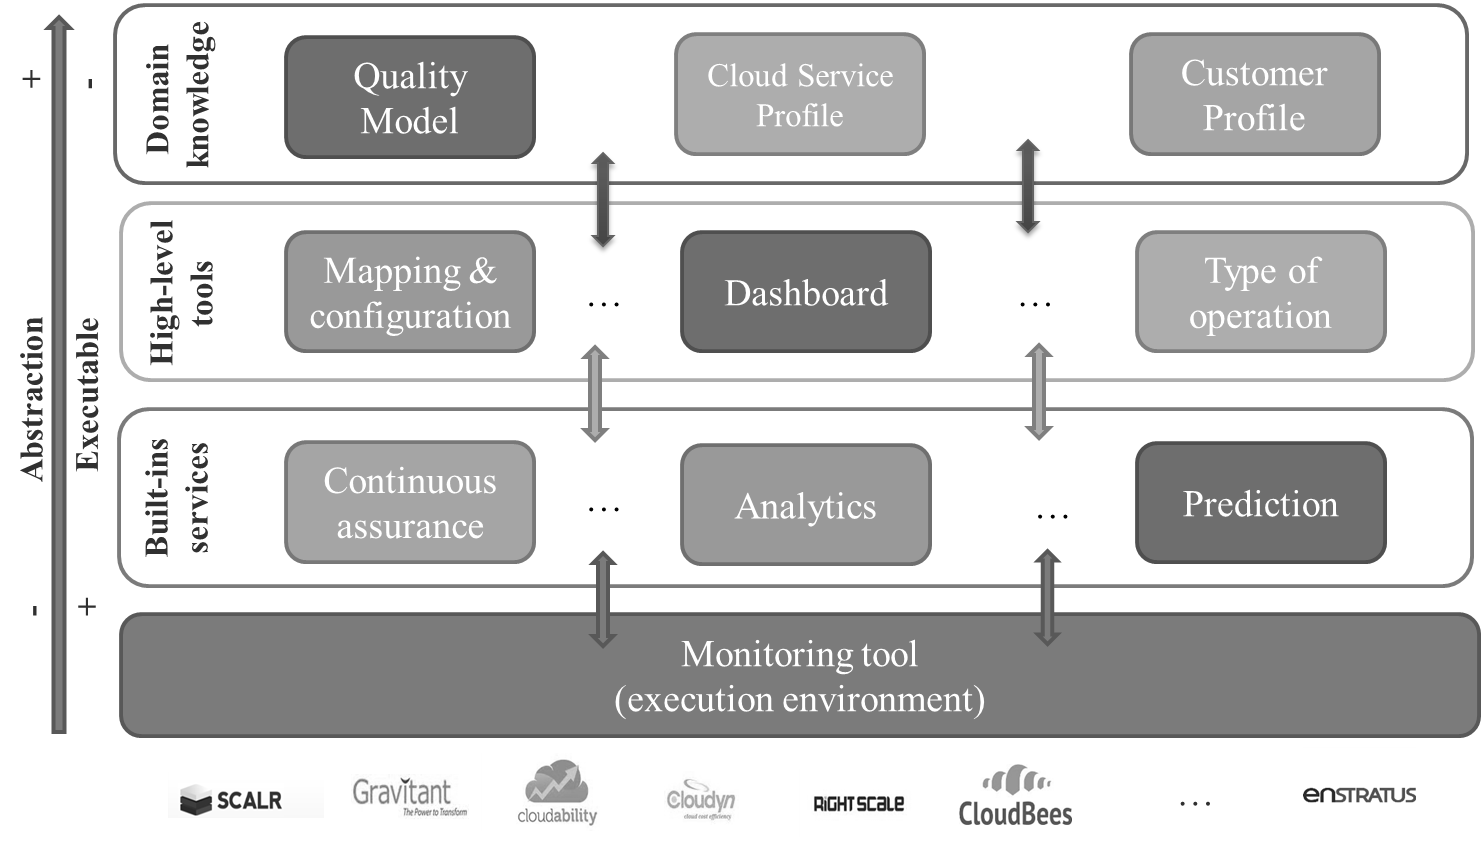
\includegraphics[width=12cm]{./imgs/qos-framework}
 \caption{QoS Framework.}
 \label{fig:qos-framework}
\end{figure}



Therefore Figure~\ref{fig:lambda-qos} depicts the building blocks and layers of the Lambda architecture with 
an adaptation to support semantics. 

\begin{itemize}
 \item \textbf{Batch layer.} It contains immutable, constantly growing dataset stored on a distributed file system like HDFS. This layer 
 receives as input the raw data coming from a queue. Data is then computed by means of some function and results are finally exposed 
 as batch views. As an extra step and with the aim of supporting the use of semantics these final views are promoted as RDF and thus SPARQL queries 
 can be executed on the computed results. This approach of adding an extra layer to ease queries over batch views has been 
 already address using SQL as a formal query language, e.g. SploutSQL. In this case SPARQL and RDF is selected to support the implicit 
 creation of queries from a semantic model. This layer is usually implemented using a MapReduce-based framework such as Apache Hadoop or 
 a more high-level framework such as Apache Pig. A final remark in this layer lies in the off-line execution of the algorithms or functions 
 that eases the pre-computation of results when large dataset processing is required.
 
 \item \textbf{Serving layer.} The responsibility of this layer is to manage both batch and real-time views 
 with the aim of providing a way of querying and merging both views and populate results to be consumed by 
 a third-service. In this case, this layer is in charge of executing the SPARQL queries (using a federated extension~\cite{DBLP:journals/corr/RakhmawatiUKHH13} 
 such as SPARQL-FedX~\cite{DBLP:conf/esws/SchwarteHHSS11}) and publish the results as RDF. At a first glance this job does not require 
 random writers but must support batch updates and random reads. In this case the implementation of joining 
 results is also designed as a Storm/Trident topology to enable and distributed real-time updates.
%  However it can be extraordinarily simple (candidates could be ElephantDB or Voldemort).

\item \textbf{Speed layer.} It deals with new data to compensate or decrease the latency of the batch layer. 
Functions are deployed on some stream processing system such as Storm, S4 or Spark and results are finally 
exposed as RDF. The functionality provided by this layer is mainly the same as the batch-layer but removing 
the latency and affording a real-time query system. Once data is also processed and available in the batch 
view a synchronization process must remove data from the real-time views. In this case Apache Zookepper 
can be used to keep synchronization in a distributed system.
\end{itemize}

The ``semantized'' Lambda Architecture using RDF and SPARQL on top of the batch and real-time views enables 
the possibility of handling the complexity of Big Data systems by defining a clear set of principles. Specifically 
the use of semantics serve to integrate data under a common data model that can be queried using a formal 
query language such as SPARQL. Furthermore immutability, human fault-tolerance and re-computation basic principles 
that can be easily adopted with the Hadoop platform. Finally and depending on the real-time requirements of 
the system some parts can be omitted and integrated in a further stage.

\begin{figure}[!ht]
\centering
	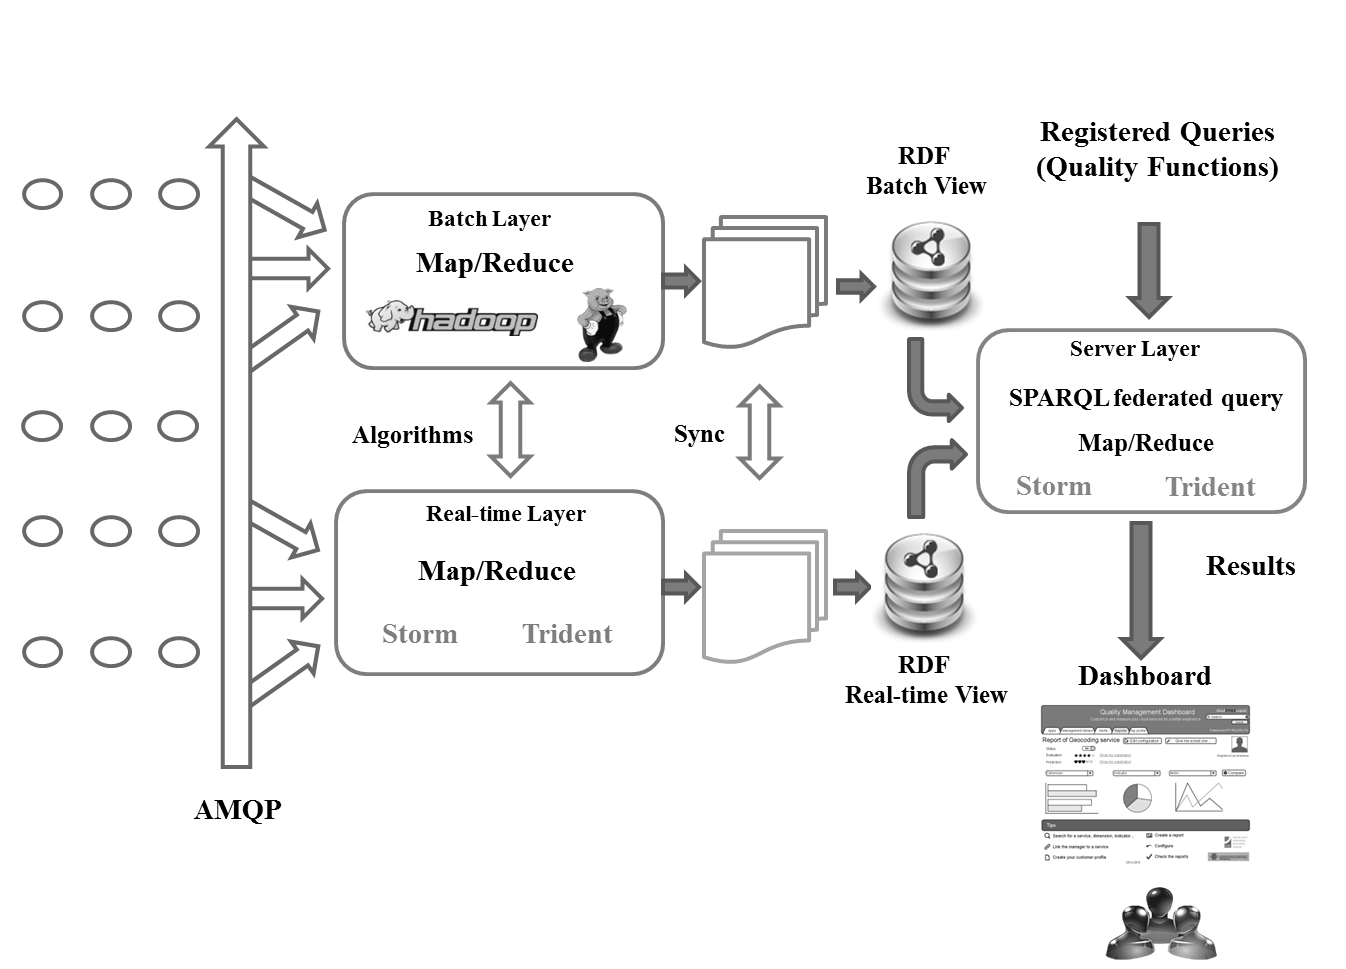
\includegraphics[width=12cm]{./imgs/lambda-qos}
 \caption{A semantic-based Lambda Architecture for real-time processing of diverse datastreams.}
 \label{fig:lambda-qos}
\end{figure}






